\begin{equation}
    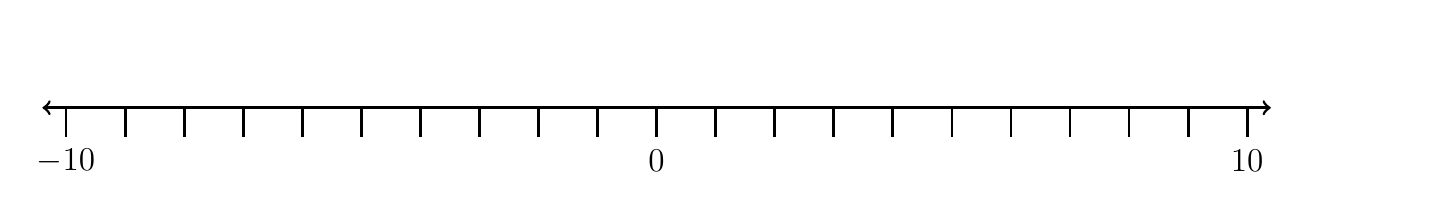
\begin{tikzpicture}[scale=0.75, baseline={([yshift=-1pt]current bounding box.north)}]
        % axis, arrow style to-to
        \draw[{To[scale=1.3]}-{To[scale=1.3]}, line width=1pt] (-10.4, 0) -- (10.4, 0);
        % tick marks
        \foreach \x in {-10,-9,...,10}
            \draw[shift={(\x,0)},color=black, line width=1pt] (0pt,-14pt) -- (0pt,0pt);
        % numbers along each axis
        \foreach \x in {-10,0,10}
            \draw[shift={(\x,-0.8)},color=black] node[font=\large,text height=12pt] {$\x$};
        % dots
        % arrow
        % equation at right end
        \node [font=\large, minimum width=30mm] at (11.0,1.2) {$  $};
    \end{tikzpicture}
\end{equation}
